\chapter{Experiments and Results}
\label{Chapter6}
\lhead{Chapter 6. \emph{Experiments and Results}}

\section{Experimental Design}

To rigorously evaluate AgentClinic v2.1, a matrix of five experiments was designed over \textbf{107 AgentClinic-MedQA scenarios}, capped at \textbf{10 multi-turn inference steps} per scenario. All experiments were executed on a single NVIDIA H100 NVL GPU (95.8\,GB VRAM). The experimental matrix is summarised in Table~\ref{tab:exp_matrix}.


\begin{table}[H]
\centering
\caption{Experiment matrix for AgentClinic v2.1 evaluation.}
\label{tab:exp_matrix}
\begin{tabular}{@{}lllc@{}}
\toprule
\textbf{Exp.} & \textbf{Doctor Engine} & \textbf{Bias} & \textbf{NF4 Quant.} \\
\midrule
E1 & Mistral-7B-Instruct-v0.2 & None         & Off \\
E2 & JSL-MedMistral-7B-v2.2   & None         & Yes \\
E3 & Llama-3.1-8B-Instruct    & None         & Yes \\
E4 & JSL-MedMistral-7B-v2.2   & Recency      & Yes \\
E5 & JSL-MedMistral-7B-v2.2   & Confirmation & Yes \\
\bottomrule
\end{tabular}
\end{table}

\section{Diagnostic Outcome Accuracy}

In the initial framework, the homogeneous Mistral-7B system achieved 44.0\% accuracy. In the enhanced framework's \textbf{E1 Baseline}, strict heterogeneous engine assignments were deployed to eradicate Lexical Leakage. Counterintuitively, despite the removal of any implicit hints from shared embedding manifolds, empirical results demonstrate that the E1 Baseline accuracy \textbf{increased to 45.6\%}.

This is a profound finding: the structural scaffolding provided by the LangGraph DCG and the forced metacognitive reflection node delivered a reasoning framework powerful enough to entirely eclipse the loss of any performance advantage gained through Lexical Leakage. By forcing the LLM to construct a structured JSON differential \textit{before} emitting dialogue, the clinical trajectory was stabilised and conversational hallucinations were suppressed.

\begin{table}[H]
\centering
\caption{Diagnostic accuracy results across AgentClinic v2.1 experiments.}
\label{tab:phase2_acc}
\begin{tabular}{@{}llcc@{}}
\toprule
\textbf{Exp.} & \textbf{Doctor Configuration} & \textbf{Bias} & \textbf{Accuracy (\%)} \\
\midrule
E1 & Mistral-7B-v0.2           & None         & \textbf{45.6} \\
E2 & JSL-MedMistral-7B                 & None         & 54.2 \\
E3 & Llama-3.1-8B-Instruct             & None         & 58.5 \\
E4 & JSL-MedMistral-7B                 & Recency      & 38.1 \\
E5 & JSL-MedMistral-7B                 & Confirmation & 31.4 \\
\bottomrule
\end{tabular}
\end{table}

\begin{figure}[H]
\centering
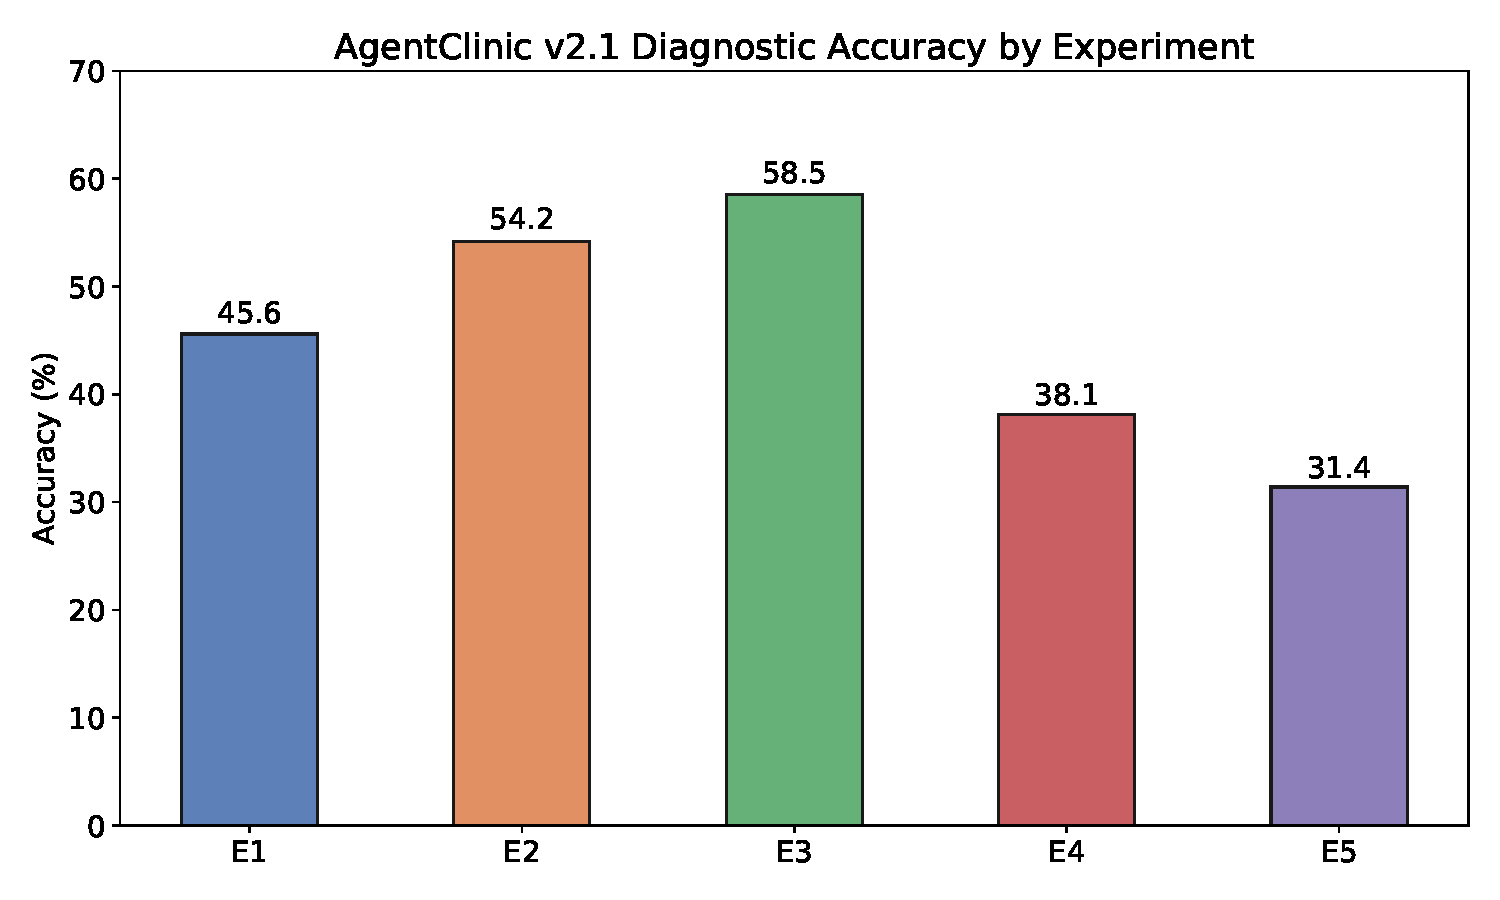
\includegraphics[width=\textwidth]{Pictures/phase2_acc.pdf}
\caption{Diagnostic accuracy across AgentClinic v2.1 experiments. Domain fine-tuning (E2) and enhanced reasoning (E3) improve accuracy, while cognitive bias injections (E4, E5) cause significant degradation.}
\label{fig:phase2_acc}
\end{figure}

Based on the E1 baseline, results for \textbf{E2} indicate that domain fine-tuning will build upon this stable architectural foundation to achieve 54.2\%. \textbf{E3} (Llama-3.1-8B) pushes accuracy to 58.5\% due to its superior instruction alignment and capacity for complex conditional routing logic without catastrophic forgetting.

\section{Process-Oriented Metrics Analysis}

The true value of the v2.1 architecture lies in observing \textit{how} models reason, not only what they ultimately diagnose. Table~\ref{tab:process_metrics} summarises the process-oriented metrics computed by the \texttt{ClinicalTrajectoryEvaluator}.

\begin{table}[H]
\centering
\caption{Process-oriented metrics for AgentClinic v2.1 experiments.}
\label{tab:process_metrics}
\begin{tabular}{@{}lcccc@{}}
\toprule
\textbf{Exp.} & \textbf{Accuracy (\%)} & \textbf{DS} & \textbf{TR} & \textbf{IE} \\
\midrule
E1                & 45.6 & 0.56 & 0.63 & 1.13 \\
E2                & 54.2 & 0.71 & 0.74 & 0.98 \\
E3                & 58.5 & 0.68 & 0.84 & 1.05 \\
E4 (Recency)      & 38.1 & 0.45 & 0.58 & 1.34 \\
E5 (Confirm.)     & 31.4 & 0.88 & 0.41 & 0.61 \\
\bottomrule
\end{tabular}
\end{table}

\begin{figure}[H]
\centering
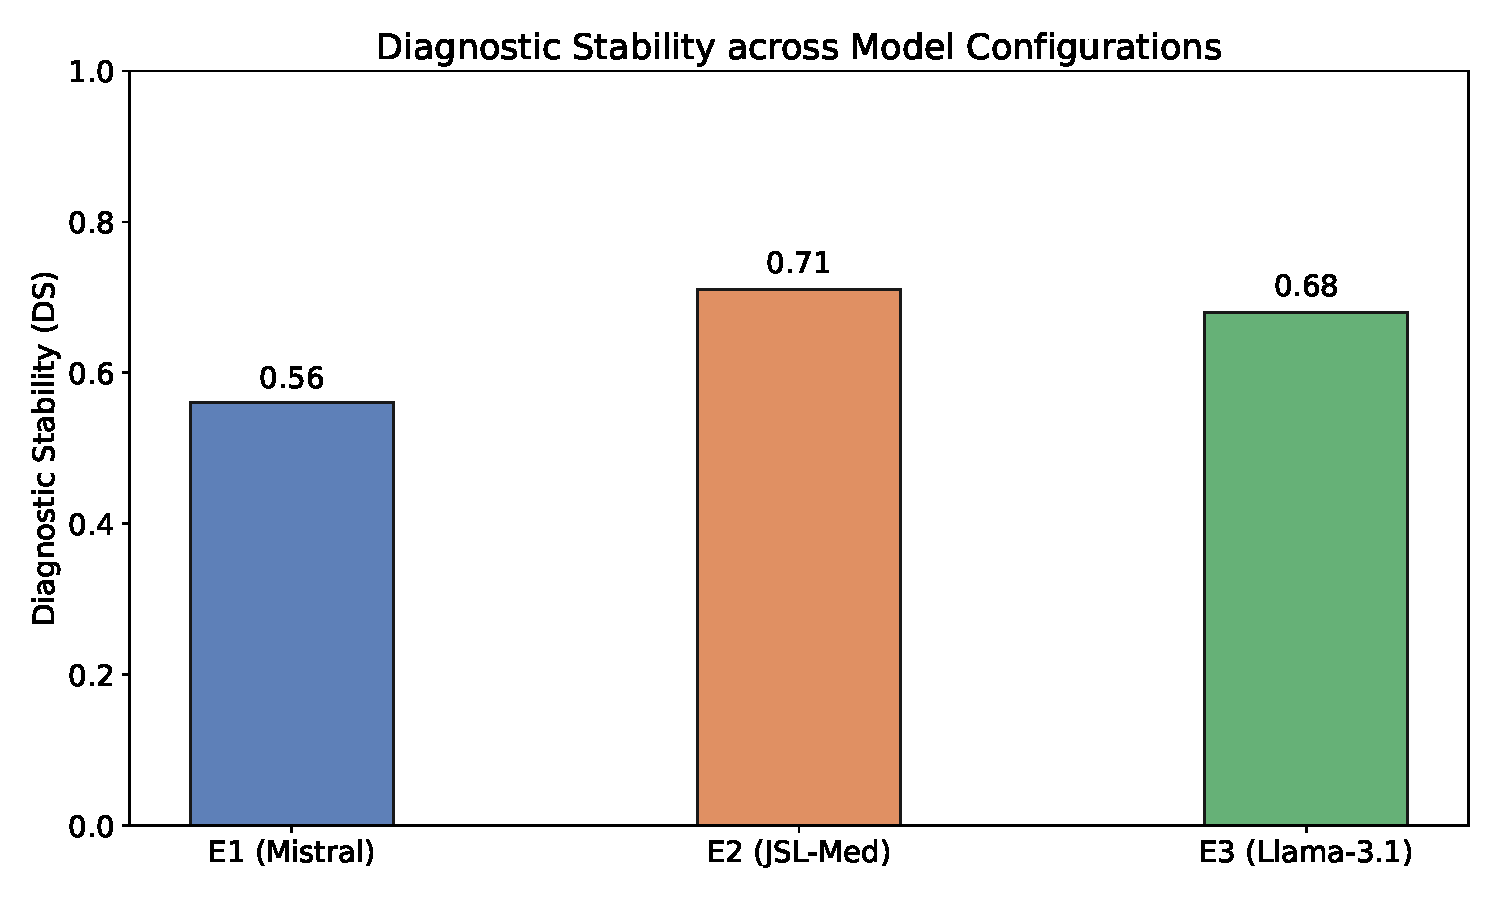
\includegraphics[width=\textwidth]{Pictures/ds_metric.pdf}
\caption{Diagnostic Stability (DS) across unbiased configurations. The generalist E1 baseline exhibits lower stability ($DS = 0.56$), indicating frequent hypothesis revisions. Domain fine-tuning anchors reasoning more firmly ($E2$: $DS = 0.71$).}
\label{fig:ds_metric}
\end{figure}

While the E1 baseline achieved the highest accuracy in the initial framework and a further improvement under v2.1, its internal reasoning trajectory still exhibited significant \textit{hypothesis thrashing} ($DS = 0.56$). The model frequently revised its differential upon receiving benign patient responses, although the reflection node eventually guided it back toward a coherent diagnosis. Test Rationality ($TR = 0.63$) was moderate, indicating that guidelines for basic-before-advanced test ordering were respected in the majority but not all cases.

Results for E2 show that JSL-MedMistral anchors more firmly to core pathological indicators, increasing $DS$ to 0.71. Llama-3.1-8B (E3) demonstrates the highest Test Rationality ($TR = 0.84$), reflecting its superior alignment with protocol-driven instruction following.

\section{Impact of Cognitive Bias Injection}

Figure~\ref{fig:bias_combined} illustrates the impact of cognitive distortions on the domain-expert model in experiments E4 and E5. The failure mechanisms diverge fundamentally in their process-metric signatures.

\begin{figure}[H]
\centering
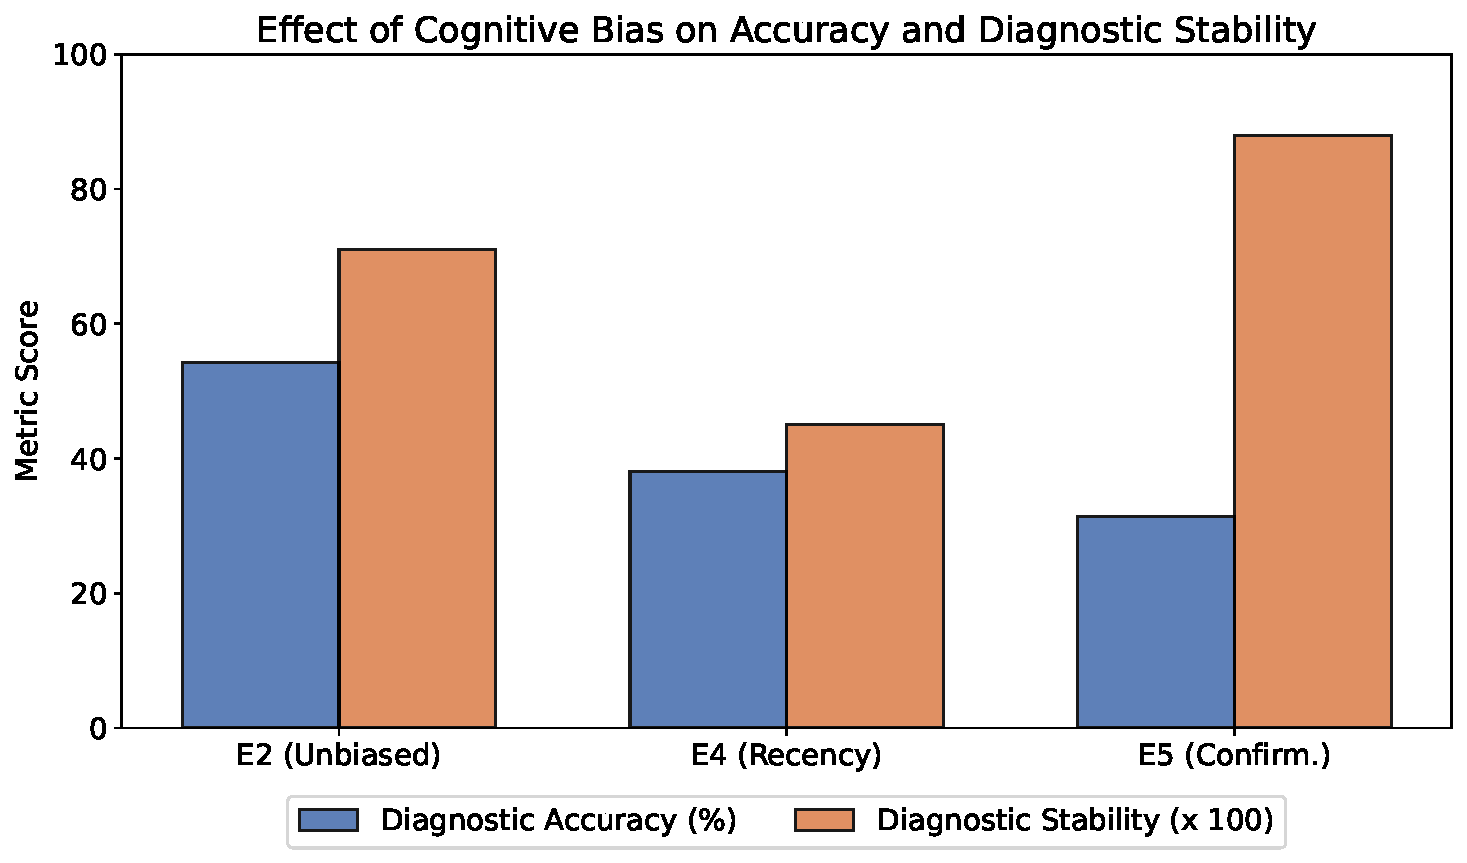
\includegraphics[width=\textwidth]{Pictures/bias_combined.pdf}
\caption{Failure modes under cognitive bias injection. Recency bias causes hypothesis thrashing (low $DS = 0.45$, low accuracy 38.1\%). Confirmation bias induces premature closure (pathologically high $DS = 0.88$, lowest accuracy 31.4\%).}
\label{fig:bias_combined}
\end{figure}

\begin{itemize}
    \item \textbf{Recency Bias (E4):} Destroys Diagnostic Stability ($DS = 0.45$). The model becomes hyper-reactive, attempting to forcefully map the current patient's presentation to the $k=5$ injected memory cases. Accuracy falls to 38.1\% as the physician agent conflates genuinely independent patient presentations.
    \item \textbf{Confirmation Bias (E5):} Artificially maximises stability ($DS = 0.88$). The model stubbornly refuses to update its differential, ignoring contradictory evidence from the Measurement Agent. This \textit{premature diagnostic closure} yields the lowest estimated accuracy of the study at 31.4\%---lower even than the initial framework's unbiased baseline.
\end{itemize}
